\chapter{Methodology} \label{Procedure}
\label{c3} % la etiqueta para referencias

\section{Context}
\label{c3:Methodology:Context}
% Maybe the following portion is more of a motivation rather than procedure.
The simulation is based on the optical setup shown in figure (\ref{fig:Simulated_Experiment}), which reproduces the existing setup in the FICA UANDES optics laboratory. It shares the core structure with other optical experiments that study, yet are not limited to, atmospheric turbulence, crosstalk and simple data transmission (Tx) and reception (Rx) analysis. However, the feature that is of most interesting for this case, is the telescope in the Rx side.

\begin{figure}[htbp]
    \centering
    \fbox{\includegraphics[width=7cm]{images/c03/Simulated_Experiment.png}}
    \caption{Diagram showing the simulated experiment.}
    \label{fig:Simulated_Experiment}
\end{figure}

\newpage
There is a myriad of telescopes, among the which the Schmidt-Cassegrain particularly stands out. It is one of the most used ones because it allows wide apertures devices to be built within a short cylinder (compared with its focal-length-equivalent refractor). The disadvantage that the Schmidt-Cassegrain encompasses, is its central obstruction ((g) in figure (\ref{fig:Simulated_Experiment})), that serves as the resting location for the mirror that reflects and focuses incoming light towards the eyepiece ((f) in figure (\ref{fig:Simulated_Experiment})). For distant targets, this obstruction is inconsequential due to the parallax effect; nevertheless, for shorter distances, such as the ones that might be used in a laboratory, it becomes an obstacle for a vortex, as it can block its central singularity.

\begin{figure}[htbp]
    \centering
    \includegraphics[width=7cm]{images/c03/Cassegrain-Obstruction.png}
    \caption{Schmidt-Cassegrain telescope like the one available in the FICA laboratory. The obstruction is colored in light yellow \protect\cite{Schmidt-Cassegrain_Pics}.}
    \label{fig:Schmidt-Cassegrain-Obstruction}
\end{figure}

The simulation takes into consideration every aspect of this experiment: creation and propagation of the phase mask, central obstruction placement and intensity and topological charge analysis at the receiving end.

Because the obstruction in figure (\ref{fig:Simulated_Experiment}) is in the receiver system (although it could be relocated if the setup is modified) the concept of staged propagation is introduced. Staged propagation is intended to model a single circular-shaped central obstruction at any location within the propagation path. This concept may also model a regular, unobstructed propagation. Briefly explained, it simulates a phase mask to be propagated through a total distance $z_f$ measured in [mm] from the beginning (Tx), that encounters an obstruction located at $z_i$, also in [mm]. The obstruction size can vary, including a null size to model unobstructed propagations.

\section{Procedure}
\label{c3:Procedure}

The simulation is made possible thanks to ten MATLAB modules: nine functions and one main script, the latter called \textit{Obs\_Analysis\_Exe.m}. Of the nine functions, eight provide distinct aspects of the simulation, such as creating a specific image or describing a mathematical function along with their variables. The remaining function is the main one, called \textit{Obstruction\_Analysis.m}, which is the actual simulation of the setup shown in figure (\ref{fig:Simulated_Experiment}), and it makes use of the other eight functions in chronological order. The main script recalls the main function to obtain results with varying parameters to test diverse scenarios.

Do consider that the purpose of the following description is to present an overview of the simulation as a whole process. For a more detailed explanation on each function and script, their arguments, code revision and documentation, please refer to appendix \ref{MATLAB_Scripts}.

First of all, a phase mask is generated. The phase mask can be that of a regular vortex, generated by the function \textit{OAMgridFullHD\_GS.m}, or a perfect vortex, generated by the function \textit{OPE\_Mask.m}. In the main function, they are represented by argument \textit{type} which can take the values 0 or 1, respectively. Both types need a topological charge specified, represented by the argument \textit{state}, to generate the non-propagated mask at said state.

Then, the staged propagation takes place. As it was discussed in section \ref{c3:Methodology:Context}, the term of staged propagation is introduced in this paper. This method is better illustrated in the flow chart shown in figure (\ref{fig:staged_propagation_flow_chart}).

\begin{figure}[htbp]
    \centering
    \fbox{\includegraphics[width=7.5cm]{images/c03/Staged_Propagation_Flux_Chart.png}}
    \caption{Staged propagation flow chart along with per-stage visualizations of the mask along the path.}
    \label{fig:staged_propagation_flow_chart}
\end{figure}

Staged propagation receives as arguments the distances \textit{z\_i} and $z_f$, which are given in [mm], and the obstruction size, which is measured in pixels (px). If a direct propagation is desired, $z_i$ should be set to 0. If an unobstructed propagation is desired, the obstruction size, represented by the variable \textit{obstruction\_radius}, should be set to 0; in this case, it is recommended to do a direct propagation.

Once the propagation is simulated, the topological charge is estimated using the function \textit{Circ\_Profile.m}, that takes an intensity profile at the pixels of a circumference with a given radius, in [px]. This circular profile is taken on the propagated mask. By counting the number of peaks that the profile has, one can estimate the topological charge. The number of peaks are the number of ``creases'' that the image has, which should be the same number as the topological charge. Theses creases look like a line, which on one side are a very light gray or white, and on the other side are dark gray or black.

This whole process returns the data to produce two figures. The first one shows four images: the phase mask just before the obstruction, the propagated phase mask, the resulting vortex and its intensity profile. From now on, these images will be respectively referred by the names: unobstructed phase mask, propagated phase mast, vortex or OAM and intensity profile. The second figure shows the plot of the circular profile taken on the propagated phase mask. Examples of these can be seen in figures (\ref{fig:example_figure1}) and (\ref{fig:example_figure2}), respectively.

\begin{figure}[htbp]
    \centering
    \includegraphics[width=10cm]{images/c03/Example_Result.eps}
    \caption{Example figure of the first kind. The sub-figures seen are, clockwise from top-left, the phase mask at the obstruction's location, the propagated phase mask, the intensity profile and the vortex. The cyan circumference in the propagated phase mask shows where the circular profile was taken. Notice that in this example, obstruction radius is 0 [px], and therefore, there is no obstruction.}
    \label{fig:example_figure1}
\end{figure}

\begin{figure}[htbp]
    \centering
    \includegraphics[width=10cm]{images/c03/TC_example.eps}
    \caption{Example figure of the second kind. Notice that this plot is from a circular profile, meaning that the far right side of the graph directly continues on the far left side.}
    \label{fig:example_figure2}
\end{figure}

\newpage
All of the main function's arguments are listed below. Once again, if a more in-depth explanation is required, please refer to appendix \ref{MATLAB_Scripts}.

\begin{enumerate}
    \item \textit{img\_size}: Size of the image in [px]. All images generated are 1:1, i.e, a square of side \textit{img\_size}.
    \item \textit{state} ($\ell$): Topological charge. An integer is expected.
    \item \textit{z\_i}: First stage propagation distance in [mm]; denoted as $z_i$ in this work.
    \item \textit{z\_f}: Total propagation distance in [mm]. Second stage propagation distance is given by $z_f - z_i$ [mm]. Denoted as $z_f$ in this work.
    \item \textit{profile\_radius}: Profile radius in [px]. Any value can be used, as long as it is lower than half the image size.
    \item \textit{type}: Type of vortex. $type = 0$ represents regular vortices and $type = 1$ perfect vortices. Any other value will produce an error.
    \item \textit{obstruction\_radius}: Obstruction radius in [px]. Values higher than 100 are not recommended.
    \item \textit{sigma} ($\sigma$): Standard deviation of the 2D Gaussian that generates regular vortices. It is used to control the size of the Gaussian, where larger values return larger beams.
    \item \textit{Rpx}: Aperture size in [px]. The main function converts this measure to [mm] internally. The expected value is 764 [px]; however, under a slightly different scenario (to be presented later on) it can be set at 500 [px].
    \item \textit{N}: Number of Bessel's zeroes\footnotemark{} and number of rings. Values expected here are integers between 30 and 60.
\end{enumerate}

\footnotetext{The function used to calculate the Bessel function's roots is \textit{besselzero.m} \cite{besselzero-MathWorks}. The function can be seen in appendix (\ref{MATLAB_Scripts}).}

Arguments (i) and (j) were inherited from Bravo's undergraduate thesis \cite{Thesis_Herbert:2020}. He established the acceptable values' range for aperture and number of rings, in order to create a perfect vortex, by following the vortex's definition: a beam with a main ring that concentrates most of the beam's light intensity and a black center region, completely absent of light. He confirmed this by taking multiple intensity profiles on the vortices produced by these values.

Other arguments are implicit within some of the functions. For instance, the image size was set to 1080x1080 [px] because the UANDES optics' laboratory SLMs (Spatial Light Modulator) has a native resolution of 1920x1080 [px] (width and height, respectively) and 1080 [px] is the smallest side. Additionally, both functions, \textit{Fresnel.m} and \textit{OAMgridFullHD\_GS.m}, consider that the wavelength of the laser used is the same as the ones available in the laboratory, $660 \times 10^{-6}$ [mm], or equivalently 660 [nm]. In a similar fashion, the circular profile's radius is fixed to a value of 200 [px]; although this value could vary depending on the size of the obstruction or some other reference, after several iterations it was concluded that a large-enough fixed value delivered more accurate estimates. The other arguments were created by the author for this work.

\section{Main Script Usage}

The objective of this section is to instruct the reader on how to use the main script and how to input the arguments to obtain results of different nature.

First, the variables of the program are prompted to the user by the MATLAB script \textit{Obs\_Analysis\_Exe.m}. It is useful to distinguish fundamental variables from scenario variables. Fundamental variables are understood to be variables that affect the vortices themselves, and do not play a role in the obstruction nor propagation. On the other hand, scenario variables are the opposite.

For regular vortices, the fundamental variable is $\sigma$, and for perfect vortices, these are $N$ and $Rpx$. For most cases, these variables are best left unchanged, as a $\sigma = 100$ generates regular vortices correctly for practically all distances, from near-field to infinity. On the other hand, Herbert's work on perfect vortices concluded that the best vortices are produced by setting $N = \{40,60\}$ and $Rpx = 764$ [px] (roughly equivalent to 6.11 [mm]). During the course of this work, it was discovered that the range of $N$ can be expanded to $\{30,60\}$ without altering the outcome negatively. It was also discovered that the $Rpx$ can also be equal to $500$ (roughly equivalent to 4 [mm]); however, in order to procure a good vortex, the total propagation distance should be increased by approximately 30\% over its value at the time of using $Rpx = 764$ [px]. But that as it may, these discoveries did not seem to provide more interesting data than what was already available. In consequence and for the purpose of this work's main results, the fundamental variables were fixed at values within the margins previously described.

Moving on to scenario variables, the program gives the user the faculty to obtain results using different combinations of values by iterating to contemplate all possible combinations of them. For instance, say that the user wants to obtain results for unobstructed vortices, regular and perfect, of $\ell = 10$, but for different propagation distances, say 500 [mm] and 1000 [mm]. They should simply separate the desired evaluation values with a space, and the program iterates over all given combinations. In that event, the results' folder will contain eight images: four for perfect vortices and other four for regular vortices. Furthermore, each propagation produces two figures: one for the phase masks, vortex and its intensity profile, and a second one for the topological charge measurement, giving a grand total of 16 images (two per vortex). Therefore, it would really be considering two scenarios for each type of vortex, just as it was expected by only varying the total propagation distance (``Stage 2 Distances'' in the window). The previous case can be extended to all sorts of combinations and scenarios considering these variables.

In general, the number of cases is given by the multiplication between the total number of types of vortex, stages 1 and 2 distances and obstruction radii. This produces twice as much images, because each scenario produces two figures.

\begin{figure}[htbp]
    \centering
    \includegraphics[scale=0.85]{images/c03/Input_Window_MATLAB_divided_v2.PNG}
    \caption{\textit{Obs\_Analysis\_Exe.m} prompt window filled out to obtain the results described above. The window was cut in half for better visualization in this document.}
    \label{fig:input_window}
\end{figure}

\newpage
Running the program with the parameters shown in figure (\ref{fig:input_window}), will result in the creation of the following folder and sub-folders, when the image format type is \textit{png}\footnote{Because Windows does not allow to preview \textit{eps} files by default, it is not necessary to classify them to preview them, as the names are self-explanatory. However, Windows does allows \textit{png} files to be previewed; in consequence, the program is designed to classify them to allow the user to scroll through the images continuously without interruptions such as showing a different type of vortex or figure.}. The images inside these folders are of the same type as figures (\ref{fig:example_figure1}) and (\ref{fig:example_figure2}).

\begin{figure}[htbp]
    \centering
    \includegraphics[width=11cm]{images/c03/General_Folder.PNG}
    \caption{Created folder (highlighted in gray) with the resulting images. Notice that its named (automatically) after the date it was created. If a folder with the same name already exists, the suffix (i) is placed, where i is the smallest available natural number.}
    \label{fig:general_folder}
\end{figure}

\begin{figure}[htbp]
    \centering
    \includegraphics[width=11cm]{images/c03/Folder.PNG}
    \caption{Inside the created folder, where the images are classified by their propagation distance.}
    \label{fig:folder}
\end{figure}

\begin{figure}[htbp]
    \centering
    \includegraphics[width=11cm]{images/c03/Specific_folder.PNG}
    \caption{View inside one of the propagation distances' folder, specifically the z=1000 for this case. At this level, the sub-folders are classified by vortex type.}
    \label{fig:specific_folder}
\end{figure}

\begin{figure}[htbp]
    \centering
    \includegraphics[width=11cm]{images/c03/Final_Folder.PNG}
    \caption{Inside one of the vortices type's folder, specifically the perfect vortices, the images are located. Their topological charges' plots are in a separate folder called ``TC''.}
    \label{fig:final_folder}
\end{figure}

\begin{figure}[htbp]
    \centering
    \includegraphics[width=11cm]{images/c03/Final_Folder_TC.PNG}
    \caption{View inside the TC folder.}
    \label{fig:final_folder_TC}
\end{figure}

\newpage
Notice that each image is named by its parameters \textit{type}, meaning the vortex's type; \textit{r}, meaning its obstruction radius; $z_i$ and $z_f$. The topological charge images are also named in this manner, with the addition of the suffix ``\_TC'' to distinguish them.

\begin{figure}[htbp]
    \centering
    \includegraphics[width=9cm]{images/c03/Console_Output.PNG}
    \caption{Part of the console output obtained from executing the program \textit{Obs\_Analysis\_Exe.m} using the parameters shown in figure (\ref{fig:input_window}).}
    \label{fig:my_label}
\end{figure}

Finally, the console output displays two types of information blocks. Each block is separated by a dashed line. The first type shows the information of the latest single cycle, including vortex type, which stage of the program was executing at the moment (prints in real time) and the total runtime of that cycle. This is the most common block type and, naturally, it appears as many times as there are cycles. The second type is the last block, and is a summary of the complete execution, showing the folder's name where the images were saved (``Saved in folder'', in the above figure), total number of images and vortices, total elapsed time and a time average per cycle.

